\documentclass[lettersize,journal]{IEEEtran}
\usepackage{rotating}
\makeatletter
\setlength{\@fptop}{0pt}
\makeatother
\usepackage{amsmath,amsfonts}
\usepackage{algorithmic}
\usepackage{algorithm}
\usepackage{array}
\usepackage[caption=false,font=normalsize,labelfont=sf,textfont=sf]{subfig}
\usepackage{textcomp}
\usepackage{stfloats}
\usepackage{url}
\usepackage{verbatim}
\usepackage{graphicx}
\usepackage{cite}
\usepackage{multirow}


\hyphenation{op-tical net-works semi-conduc-tor IEEE-Xplore}
\def\BibTeX{{\rm B\kern-.05em{\sc i\kern-.025em b}\kern-.08em
    T\kern-.1667em\lower.7ex\hbox{E}\kern-.125emX}}
\usepackage{balance}
% updated with editorial comments 8/9/2021

\begin{document}

\title{Enhancing Molecular Generation with\\FragGPT-Guided Genetic Algorithms}

\author{Tiangai Yao, Zhangfan Yang, Junkai Ji,~\IEEEmembership{Member,~IEEE}\\
        % <-this % stops a space
\thanks{T. Yao, Z. Yang, and J. Ji are with the College of Computer Science and Software Engineering, Shenzhen University, Shenzhen 518060, China (e-mail: 2400671005@mails.szu.edu.cn; yangzhangfan@szu.edu.cn; jijunkai@szu.edu.cn).}% <-this % stops a space
\thanks{Manuscript received December 15, 2024; revised January 20, 2025.}}
% The paper headers
\markboth{IEEE Transactions on Evolutionary Computation,~Vol.~XX, No.~X, Month~2025}%
{Yao \MakeLowercase{\textit{et al.}}: Enhancing Molecular Generation with FragGPT-Guided Genetic Algorithms}

\IEEEpubid{1089-778X/25\$31.00~\copyright~2025 IEEE}
% Remember, if you use this you must call \IEEEpubidadjcol in the second
% column for its text to clear the IEEEpubid mark.

\maketitle
%摘要
\begin{abstract}
De novo molecular design poses a significant challenge in drug discovery, necessitating a delicate balance between exploring vast chemical spaces and targeting promising regions for optimization. This paper introduces FragGPT-GA, a novel hybrid evolutionary framework that synergistically combines a Genetic Algorithm (GA) with a Generative Pre-trained Transformer (GPT) to address this challenge. The core of our approach lies in using the GA for fine-grained structural optimization, while leveraging a fragment-based GPT model as an intelligent diversity generation operator. Specifically, the GPT model generates novel molecular candidates from masked fragments of the parent population, injecting high-quality and diverse individuals into the evolutionary loop. This mechanism enhances the exploratory capabilities of the GA, effectively preventing premature convergence to local optima. We demonstrate through comprehensive experiments, targeting a specific protein, that FragGPT-GA significantly outperforms traditional GA-only baselines in the generation of molecules with superior docking scores, drug-likeness (QED), and synthetic accessibility (SA). Our framework provides a powerful and robust strategy for efficient molecular discovery and optimization. 
\end{abstract}

\begin{IEEEkeywords}
Evolutionary Computation, Genetic Algorithm, Generative Pre-trained Transformer (GPT), De Novo Drug Design, Molecular Optimization, Hybrid Intelligence.
\end{IEEEkeywords}

\section{Introduction}
\IEEEPARstart{T}{h}e discovery of novel therapeutics is a cornerstone of modern medicine and a primary objective in computer-aided drug design (CADD). Traditional approaches, such as high-throughput virtual screening and molecular docking, have long accelerated this process by screening extensive chemical libraries for compounds active against new therapeutic targets. Although this paradigm has proven effective, it inherently confines research to a predefined and limited chemical space. As pharmaceutical companies and research institutions exhaustively screen these compound libraries, finding novel, patentable, and active compounds becomes increasingly difficult, thus necessitating innovative approaches that can explore uncharted regions of chemical space.

To address this challenge, de novo molecular generation has emerged as a promising alternative. Among various strategies, evolutionary algorithms (EAs) are a prominent approach to molecular optimization. These methods iteratively modify a population of molecules through crossover and mutation operators to optimize a predefined fitness function. This function typically combines desired properties such as binding affinity, solubility, and synthetic accessibility. A key advantage of EAs is their ability to explicitly encode chemical rules and reaction-based transformations into evolutionary operators, thereby ensuring chemical validity and synthetic feasibility. However, EAs rely on initial populations drawn from existing databases and largely perform refinements of known fragments, thereby limiting the discovery of novel scaffolds and reducing diversity, which can lead to premature convergence. 

% 添加雷达图
\begin{figure}[!t]
\centering
\includegraphics[width=3.5in]{radar.png}
\caption{Multi-objective performance comparison across key baseline methods. FragGPT-GA demonstrates superior performance with better balance across all metrics: binding affinity, drug-likeness (QED), synthetic accessibility, and novelty. The radar chart illustrates that FragGPT-GA achieves the best overall performance profile compared to RGA\cite{fuReinforcedGeneticAlgorithm}, AutoGrow4.0\cite{spiegelAutoGrow4OpensourceGenetic2020}, and MARS\cite{xie2021marsmarkovmolecularsampling} baselines.}
\label{fig:radar_comparison}
\end{figure}

\IEEEpubidadjcol 
The profound success of deep generative models in fields such as computer vision and natural language processing has inspired their application to molecular design. These sequence-based and three-dimensional (3D) structure–based models learn the underlying data distributions of large-scale chemical datasets to generate novel molecules. Sequence-based models, such as recurrent neural networks (RNNs) and Transformer architectures, represent molecules as strings (Simplified Molecular Input Line Entry System (SMILES)) and can generate diverse and novel molecules. However, the linear SMILES representation can miss contextual relationships among functional groups, and imposing complex grammars may reduce the validity of generated outputs. By contrast, 3D structure-based models, such as variational autoencoders (VAEs) and denoising diffusion probabilistic models (DDPMs), learn distributions over spatial atomic coordinates to generate molecular conformations, enabling the creation of chemically valid and structurally novel molecules with high fidelity. However, these models do not readily leverage the vast sequence-based chemical knowledge base, and their generalization can be constrained by limited 3D training data. This reveals a critical requirement for hybrid methods that combine the robust, goal-oriented optimization of Evolutionary Algorithms (EAs) with the powerful exploration and distribution-learning capabilities of deep generative models.

We propose FragGPT-GA, a generative paradigm that tightly integrates a fragment molecular language prior with multi-objective evolutionary optimization in fragment space. FragGPT-GA first trains a fragment-based molecular language model, FragGPT, to learn substructural-level statistical co-occurrence and chemical semantics from a large-scale molecular corpus. This semantic prior is injected into the mutation operator of the genetic algorithm (GA) to generate candidate fragments via semantically consistent replacement or splicing, thereby expanding the accessible chemical space while ensuring chemical validity. At the optimization stage, we systematically evaluate objective functions and show that Non-dominated Sorting Genetic Algorithm II (NSGA-II\cite{deb2002fast}) yields more drug-like molecules with higher affinity for the target. Unlike loosely coupled approaches that use language models only as a candidate pool, FragGPT-GA directly reshapes the distribution of mutation operations and the accessible chemical space. It enhances semantic coherence and structural diversity of fragment replacements while maintaining chemical validity and synthetic feasibility, thereby mitigating premature convergence. In target-based molecular generation, FragGPT-GA outperforms rule-based GAs on affinity, drug-likeness, and synthetic feasibility, and it converges faster. Furthermore, it achieves competitive performance compared with state-of-the-art deep generative models. We believe this work is a significant step toward unifying evolutionary computation with language-model-guided generation to accelerate innovation in drug discovery.
%相关工作
%-----------------------------------------------------------------------------------------------------------------------
\section{Related Work}
De novo molecular design has become a key direction in computational drug discovery, with diverse methods proposed to explore chemical space and optimize drug-related properties. Existing approaches can be broadly categorized into two groups: genetic algorithm (GA)–based methods and non-GA methods.

\subsection{GA-based methods}
GA-based approaches directly search the discrete chemical space through evolutionary operators such as crossover and mutation. Representative works include Graph-GA\cite{jensenGraphBasedGeneticAlgorithm2019}, GA+D\cite{nigamAugmentingGeneticAlgorithms2020}, GEGL\cite{ahnGuidingDeepMolecular2020}, GEAM\cite{lee2023drug}, Genetic GFN\cite{kim2024genetic}, AutoGrow 4.0\cite{spiegelAutoGrow4OpensourceGenetic2020}, RGA\cite{fuReinforcedGeneticAlgorithm}, and f-RAG\cite{lee2024molecule}. These frameworks enhance optimization efficiency by integrating discriminators, deep generative models, adversarial learning, or reinforcement signals into the GA pipeline. However, they still face common challenges, including limited scalability, instability in hybrid components (e.g., GANs or reward functions), and reduced chemical diversity due to premature convergence or local optima.

\subsection{Non-GA methods}
In contrast, non-GA methods primarily rely on deep generative modeling or reinforcement learning to imitate molecular distributions and optimize desired properties. Examples include hierarchical generative models such as JT-VAE\cite{jinJunctionTreeVariational2018} and HierVAE\cite{jin2020hierarchical}, reinforcement learning–based approaches like REINVENT\cite{olivecronaMolecularDeNovoDesign2017}, MORLD\cite{jeon2020autonomous}, RationaleRL\cite{jinMultiObjectiveMoleculeGeneration2020}, FREED\cite{yang2021hit}, and MolDQN\cite{zhou2019optimization}, as well as variational and diffusion-inspired models such as PS-VAE\cite{kong2022molecule}, MOOD\cite{lee2023exploring}, and Gen3D\cite{luoGraph2022}. Other strategies include fragment retrieval frameworks such as RetMol\cite{wang2022retrieval} and virtual screening baselines\cite{graff2021accelerating}. While these methods excel in learning chemical distributions and producing novel structures, they suffer from issues such as reward sensitivity, low sample efficiency, reliance on predefined vocabularies or motif dictionaries, and high computational demands, particularly in 3D generation or multi-objective settings.
\noindent Despite these advances, existing GA-based and non-GA methods still face critical limitations, including reduced diversity due to premature convergence, instability in hybrid architectures, low sample efficiency of reinforcement learning, and high computational costs in multi-objective and 3D settings. These challenges highlight the need for a more integrated framework that can simultaneously balance exploration and exploitation, preserve chemical validity, and achieve robust multi-objective optimization. Our proposed \textbf{FragGPT-GA} addresses these gaps by tightly coupling fragment-based generative modeling with evolutionary optimization, offering both improved performance and broader applicability in \textit{de novo} drug design.

% III. 方法 (The Proposed FragGPT-GA Framework)
% ---------------------------------------------------------------------------------------------------------------------------------
%模型提出
\section{The Proposed FragGPT-GA}
%框架介绍
\subsection{Framework Overview}
FragGPT-GA is a tightly coupled hybrid framework developed to overcome the limitations of conventional GAs and fragment-based generative models. As illustrated in Fig.~\ref{fig: flowchart}, the framework operates through a multi-stage iterative process in which each generation cycle comprises five interconnected phases: (1) \textit{fragment-based molecular decomposition}, (2) \textit{intelligent GPT-driven diversity generation}, (3) \textit{population-aware genetic operations}, (4) \textit{multi-objective fitness evaluation}, and (5) \textit{Pareto-optimal selection}. The core innovation is to integrate a fragment-aware GPT directly into the GA’s evolutionary loop, thereby bridging the gap between exploration and exploitation. Within each generation, the GA drives optimization through selection and variation, while the GPT functions as a diversity-oriented operator by generating novel candidate molecules from masked molecular fragments of the current population. This mechanism allows our framework to effectively bridge the gap between exploration and exploitation, leveraging the GA for focused optimization while utilizing the GPT to introduce diverse, high-quality structures, ultimately leading to a more balanced and superior performance profile across multiple objectives.
% 流程图
\begin{figure*}[!t]
\centering
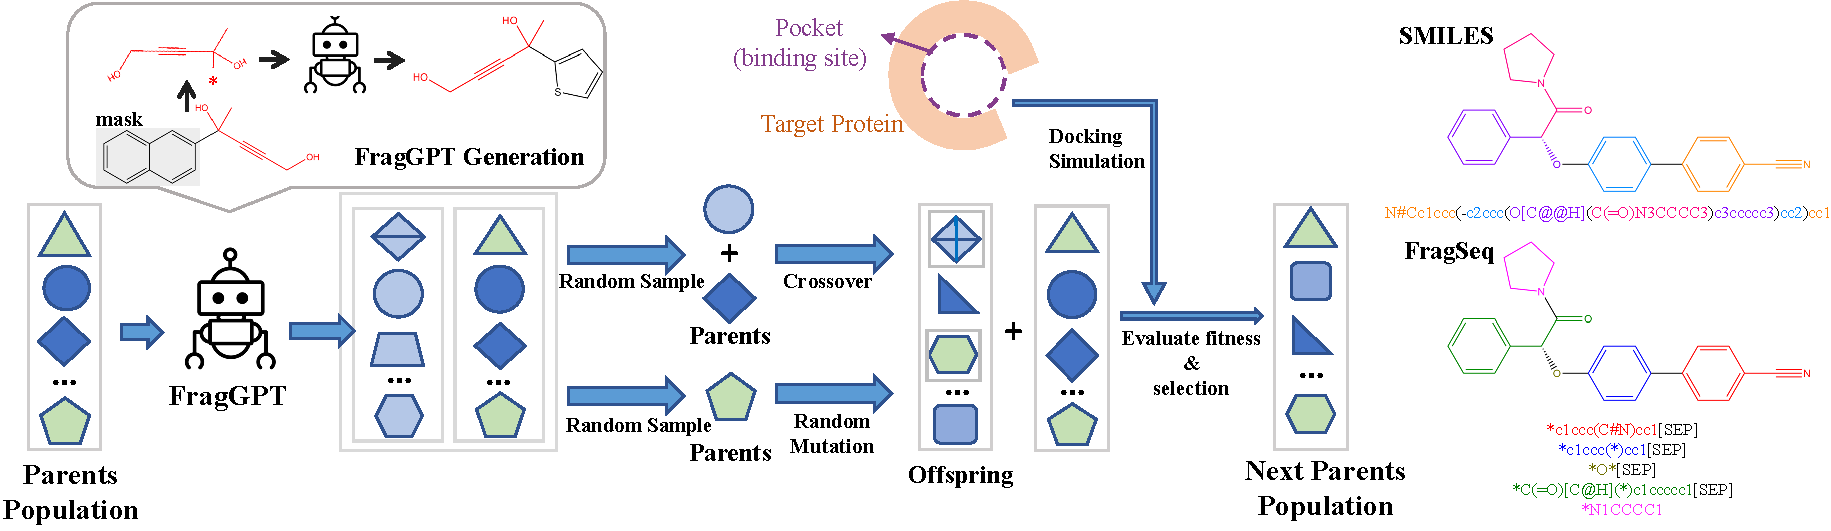
\includegraphics[width=\textwidth]{model.pdf}
\caption{The iterative workflow of the proposed FragGPT-GA framework. The process synergizes a Genetic Algorithm (GA) for optimization with a Generative Pre-trained Transformer (GPT) for diversity expansion, featuring dynamic fragment masking and multi-objective selection.}
\label{fig:flowchart}
\end{figure*}
%GPT 和 掩码
\subsection{Fragment-Based GPT and Dynamic Masking}
FragGPT-GA operates by first representing molecules in a fragment-based molecular representation, FragSeq, a fragment-level molecular language derived from the standard SMILES. To construct a FragSeq representation, a molecule is systematically deconstructed into a sequence of fragments following the Bond-Retrosynthesis-In-Combination-Strategy (BRICS) rules. BRICS defines a finite set of chemical environments to select synthetically plausible cleavage sites and to retain attachment labels, ensuring that the resulting fragments are chemically valid and stitchable. This decomposition process transforms a non-sequential graph structure into an ordered sequence of fragments, processed from left to right. An illustrative example of this conversion from a SMILES string to its corresponding FragSeq is provided in Fig.~\ref{fig:flowchart}. This sequential format is particularly advantageous as it allows a language model to naturally capture the contextual and syntactical relationships between constituent fragments within a molecule.

The FragGPT model is a generative pre-trained transformer designed to operate on the FragSeq representation. It learns the underlying chemical rules and statistical distribution of molecular structures from a large dataset. The model functions autoregressively, generating a new molecule fragment by fragment. Given a sequence of preceding fragments, FRAGPT predicts the probability distribution for the next fragment, thereby extending the molecular structure sequentially. This generative process for a molecule $m$, composed of a sequence of $L$ fragments $(f_1, f_2, ..., f_L)$ can be formally expressed as the product of conditional probabilities:
\begin{equation}
p_{\theta}(m)=\prod_{t=1}^{T} p_{\theta}\!\left(f_i \,\middle|\, f_{<i}\right),
\end{equation}
where $f_i$ is the $i$-th fragment, $f_{<i}$ represents the sequence of all preceding fragments $(f_1,...,f_{i-1})$. By sampling from these learned distributions, FragGPT can assemble novel molecules that adhere to valid chemical principles. In our framework, FragGPT is utilized to generate a new population of molecules based on the existing population from the genetic algorithm, serving as a sophisticated and chemically aware operator for generating offspring.

Another key point in FragGPT-GA is the introduction of a dynamic masking mechanism to adaptively control the influence of the FragGPT model throughout the evolutionary process. This mechanism governs the degree of structural modification by determining the number of fragments to be masked (and subsequently regenerated by FragGPT) in a given molecule. This relationship is defined by the following equation:
\begin{equation}
n_{mask}(g) = n_{initial} + \frac{g-1}{G_{max}-1} \cdot (n_{final} - n_{initial})
\end{equation}
where $g$ represents the current generation, $G_{max}$ is the maximum number of generations, $n_{initial}$ is the number of fragments masked in the first generation, and $n_{final}$ is the number of fragments masked in the final generation. This strategy establishes a clear schedule for the algorithm's behavior. In the early stages of evolution (when $g$ is small), the masking ratio is high ($n_{mask}(g) \approx n_{initial}$). This encourages FragGPT to generate substantially new molecular scaffolds by replacing large portions of the parent molecules, promoting broad \textbf{exploration} of the chemical space. As the algorithm progresses towards later generations (as $g \to G_{max}$), the masking ratio decreases ($n_{mask}(g) \to n_{final}$). Consequently, FragGPT performs more localized and subtle modifications, fine-tuning the existing molecular structures to optimize their properties. This later phase emphasizes \textbf{exploitation}, refining promising candidates rather than making radical changes. This adaptive approach allows FragGPT-GA to effectively balance the discovery of novel structures with the optimization of existing ones.
%种群GA
\subsection{Population-Aware Genetic Operations}

Following GPT-based diversity generation, the framework performs sophisticated genetic operations on an expanded population pool $P_{expanded} = P_g \cup P_{GPT}$, where $P_{GPT}$ represents the set of GPT-generated molecules. This expanded pool serves as the input for both crossover and mutation operations, enabling the genetic operators to work with a more diverse and potentially higher-quality substrate.

\noindent \textbf{Enhanced Crossover Operations:} Our crossover mechanism employs a fragment-aware approach that preserves chemically meaningful substructures while enabling recombination of beneficial motifs from different molecules. The process operates at the fragment level, ensuring that the resulting offspring maintain chemical validity and synthetic feasibility.

\noindent \textbf{Chemical-Context Mutation:} The mutation operator incorporates chemical knowledge to perform context-appropriate modifications. Rather than random SMILES string manipulations, mutations are guided by chemical rules and synthetic feasibility constraints, increasing the likelihood of generating viable compounds.
%多目标优化
\subsection{Multi-Objective Fitness Evaluation and Optimization}

The framework employs a comprehensive multi-objective fitness function that simultaneously optimizes three critical pharmaceutical properties:

\begin{equation}
F(m) = [DS(m), QED(m), SA(m)]
\end{equation}

where $DS(m)$ represents the docking score (to be minimized), $QED(m)$ quantifies drug-likeness (to be maximized), and $SA(m)$ measures synthetic accessibility (to be minimized). This multi-objective formulation ensures that optimization does not sacrifice drug-like properties or synthetic feasibility in pursuit of binding affinity alone.

The docking evaluation employs AutoDock Vina\cite{trott2010autodock} with standardized protocols, utilizing grid-based molecular docking to assess binding affinity against target proteins. The QED (Quantitative Estimate of Drug-likeness) incorporates multiple pharmaceutical properties including molecular weight, lipophilicity, and topological polar surface area. The SA score estimates synthetic accessibility based on fragment contributions and structural complexity.
%帕累托最优选择
\subsection{Pareto-Optimal Selection via NSGA-II\cite{deb2002fast}}

Selection operates under the NSGA-II\cite{deb2002fast} (Non-dominated Sorting Genetic Algorithm II) framework, which maintains population diversity while driving convergence toward the Pareto-optimal front. The algorithm performs non-dominated sorting to identify solution fronts, followed by crowding distance calculation to preserve diversity within each front.

The selection process ensures that the framework maintains a balanced portfolio of solutions representing different trade-offs between the three objectives. This approach prevents the optimization from converging to a single-objective optimum and provides medicinal chemists with diverse options for further development.
%算法描述
\subsection{Algorithmic Implementation and Computational Efficiency}

The complete FragGPT-GA algorithm is presented in Algorithm~\ref{alg:frag-gpt-ga}. The implementation features several efficiency optimizations: (1) \textit{parallel evaluation} of molecular properties using multiprocessing, (2) \textit{incremental learning} where the GPT model can optionally be fine-tuned on successful molecules from previous generations, and (3) \textit{adaptive resource allocation} that dynamically adjusts computational resources based on population convergence metrics.

\begin{algorithm}[!t]
\caption{FragGPT-GA Complete Framework}
\label{alg:frag-gpt-ga}
\begin{algorithmic}
\STATE \textbf{Input:} Initial population $P_0$, max generations $G_{max}$, GPT model $\theta$
\STATE \textbf{Output:} Pareto-optimal population $P^*$
\STATE Initialize population $P_0$ and evaluate $F(P_0)$
\FOR{$g = 1$ to $G_{max}$}
    \STATE // Fragment-based decomposition and masking
    \STATE $n_{mask} \leftarrow$ CalculateDynamicMask($g$, $G_{max}$)
    \STATE $M_g \leftarrow$ DecomposeAndMask($P_{g-1}$, $n_{mask}$)
    \STATE // GPT-powered diversity generation
    \STATE $P_{GPT} \leftarrow$ GPTGenerate($M_g$, $\theta$)
    \STATE // Population-aware genetic operations
    \STATE $P_{pool} \leftarrow P_{g-1} \cup P_{GPT}$
    \STATE $C_{cross} \leftarrow$ FragmentAwareCrossover($P_{pool}$)
    \STATE $C_{mut} \leftarrow$ ChemicalContextMutation($P_{pool}$)
    \STATE $C_g \leftarrow$ ChemicalFilter($C_{cross} \cup C_{mut}$)
    \STATE // Multi-objective evaluation
    \STATE Evaluate $F(C_g)$ = $[DS(C_g), QED(C_g), SA(C_g)]$
    \STATE // Pareto-optimal selection
    \STATE $P_g \leftarrow$ NSGA-II-Select($P_{g-1} \cup C_g$)
\ENDFOR
\STATE \textbf{return} Non-dominated solutions from $P_{G_{max}}$
\end{algorithmic}
\end{algorithm}

The modular architecture facilitates reproducibility and enables systematic ablation studies. Each component—fragment decomposition, GPT generation, genetic operations, evaluation, and selection—operates as an independent module with well-defined interfaces, allowing for easy customization and extension of the framework.


% IV. 实验设置 (Experimental Setup)
% ----------------------------------------------------
\section{Experimental Setup}
\subsection{Datasets and Docking Protocol}
In our experiments, we utilized the ZINC\cite{doi:10.1021/acs.jcim.5b00559} database, a large-scale repository of chemical compounds(around 250 thousands druglike molecules). Following the procedure in AutoGrow4.0\cite{qingfuzhangMOEAMultiobjectiveEvolutionary2007}, the molecules were stratified into four groups according to their molecular weights: $<$100, 100–150, 150–200, and 200–250 Da. FragGPT-GA then randomly sampled 250 molecules from these groups in the ratio of 2:3:4:1, respectively. The purpose of using this random sampling strategy is to ensure that the sampled molecules are not all excessively large (which would limit their potential for evolution) nor all excessively small (which would lack the necessary chemical properties), while also maintaining a balanced distribution in the initial population. Our results further demonstrate that optimizing the population by iterative crossover and mutation is largely independent of the initial population composition\cite{spiegelAutoGrow4OpensourceGenetic2020}. For our model, introducing GPT does not cause the outcomes to depend on differences in the population sampling procedure. In other words, the configuration of the initial population does not affect the final optimization convergence of the model(Evidence for this is provided in the subsequent ablation studies.).To ensure fair comparison with other baselines, we selected the same set of 10 disease-related protein targets, including G-protein-coupled receptors (GPCRs) and kinases from the DUD-E\cite{mysinger2012directory} benchmark, as well as the SARS-CoV-2 main protease\cite{shi2020graphaf}.for all the selected target protein, the binding pocket size for all the targets are set to (15.0, 15.0, 15.0). The units of coordinate are Angstrom \AA\,($10^{-10}$)m).\cite{fuReinforcedGeneticAlgorithm} For all baseline methods, molecular structures were processed with MGLTools and subsequently docked using AutoDock Vina\cite{trott2010autodock}. The resulting Vina scores were employed to evaluate the quality of the generated molecules.
%评估指标的描述  %新颖性%多样性%类药性 可合成性
\subsection{Evaluation Metrics}
Our model's performance was evaluated based on the following metrics, which assess both the overall quality of the generated set and the properties of individual molecules:
\begin{enumerate}
    \item \textbf{Novelty}: To evaluate the generative capacity of the model, we compute the novelty score, defined as the fraction of generated molecules not present in the initial population. A higher novelty value reflects the model’s ability to explore novel regions of chemical space beyond memorization.
    \item \textbf{Diversity}: The chemical diversity of the generated molecules is quantified by the average pairwise Tanimoto similarity between their 2048-bit Morgan fingerprints\cite{you2018graph}. Specifically, let $\mathcal{M}$ denote the set of generated molecules. We define
    \begin{equation}
        \mathrm{diversity} = 1 - \frac{1}{|\mathcal{M}|(|\mathcal{M}| - 1)} \sum_{m_a,m_b \in \mathcal{M}} \mathrm{sim}(m_a, m_b),
    \end{equation}    
    where $\mathrm{sim}(m_a,m_b)$ is the Tanimoto similarity between molecules $m_a$ and $m_b$. The similarity between any two molecules $X$ and $Y$ is given by $\mathrm{sim}(X,Y) = \frac{\mathbf{FP}_X^\top \mathbf{FP}_Y}{\|\mathbf{FP}_X\|_2\,\|\mathbf{FP}_Y\|_2}$, where $\mathbf{FP}_X$ and $\mathbf{FP}_Y$ are the 2048‑bit binary Morgan fingerprint vectors for $X$ and $Y$, respectively. This definition measures structural dissimilarity across the generated set and ensures that the model does not collapse toward limited structural motifs but instead produces a broad range of compounds.
    \item \textbf{Drug-likeness and Synthetic Accessibility}: Each generated molecule is further evaluated for its pharmaceutical potential. The Quantitative Estimate of Drug-likeness (QED), ranging from 0 to 1, is used to quantify how closely a compound aligns with typical drug-like properties. In parallel, the Synthetic Accessibility (SA) score, ranging from 1 (easily synthesizable) to 10 (difficult to synthesize), estimates the feasibility of practical synthesis based on fragment contributions\cite{ertl2009estimation} and structural complexity. Both QED and SA are computed using the RDKit\cite{landrum2006rdkit} toolkit(\url{http://www.rdkit.org/}).
    \item \textbf{Docking Score}: To assess binding affinity to protein targets, we use the AutoDock Vina\cite{trott2010autodock} as an evaluation metric.The resulting docking score, referred to as the Vina score, approximates the change in free energy during ligand–target binding in units of kcal/mol. Vina scores are typically negative, and more negative values correspond to stronger binding affinity between ligand and target. Lower Vina scores indicate stronger predicted binding interactions and are therefore more desirable. This score provides a direct link between generative outcomes and biological relevance.  
\end{enumerate}


% V. 结果与讨论 (Results and Discussion)
% ----------------------------------------------------
\section{Results and Discussion}
%第一个实验部分 subsection
\subsection{Comparison with Genetic Algorithm and Generative Baselines}
To rigorously evaluate the performance of our proposed method, we first conducted a comparative analysis against a comprehensive set of baseline algorithms spanning several major paradigms in molecular optimization. The selected methods include: the search-based algorithm (Screening\cite{graff2021accelerating}); generative model-based approaches such as JT-VAE and GEN3D\cite{luoGraph2022}; genetic algorithms including GA+D\cite{nigamAugmentingGeneticAlgorithms2020}, Graph-GA\cite{jensenGraphBasedGeneticAlgorithm2019}, and AutoGrow4.0\cite{spiegelAutoGrow4OpensourceGenetic2020}; reinforcement learning strategies like MolDQN\cite{zhou2019optimization}, RationaleRL\cite{jinMultiObjectiveMoleculeGeneration2020}, REINVENT\cite{olivecronaMolecularDeNovoDesign2017}, and GEGL\cite{ahnGuidingDeepMolecular2020}; and the Markov Chain Monte Carlo method, MARS\cite{xie2021marsmarkovmolecularsampling}. To ensure a fair and direct comparison of optimization efficiency, each method was strictly limited to a budget of 1000 scoring function evaluations. The performance of each algorithm was quantified by the average docking score of the top-1, top-10, and top-100 unique molecules generated during the optimization process.The overall docking performance and other‑objective metrics are summarized in Tables~\ref{tab:docking_scores} and \ref{tab:diversity_metrics}, respectively.
% Table II: Docking scores
\begin{table}[!t]
    \caption{Docking Score Comparison (kcal/mol, ↓ better)}
    \label{tab:docking_scores}
    \centering    
    \small
    \setlength{\tabcolsep}{4pt}
    
    \begin{tabular}{l c c c}
        \hline\hline
        Method & TOP-100$\downarrow$ & TOP-10$\downarrow$ & TOP-1$\downarrow$ \\
        \hline
        screening\cite{graff2021accelerating} & -9.351$\pm$0.643 & -10.433$\pm$0.563 & -11.400$\pm$0.630 \\
        MARS\cite{xie2021marsmarkovmolecularsampling} & -7.758$\pm$0.612 & -8.875$\pm$0.711 & -9.257$\pm$0.791 \\
        MolDQN\cite{zhou2019optimization} & -6.287$\pm$0.396 & -7.043$\pm$0.487 & -7.501$\pm$0.402 \\
        GEGL\cite{ahnGuidingDeepMolecular2020} & -9.064$\pm$0.920 & -9.910$\pm$0.990 & -10.450$\pm$1.040 \\
        REINVENT\cite{olivecronaMolecularDeNovoDesign2017} & -10.181$\pm$0.441 & -11.234$\pm$0.632 & -12.010$\pm$0.833 \\
        RationaleRL\cite{jinMultiObjectiveMoleculeGeneration2020} & -9.233$\pm$0.920 & -10.834$\pm$0.856 & -11.642$\pm$1.102 \\
        JTVAE\cite{jinJunctionTreeVariational2018} & -9.291$\pm$0.702 & -10.242$\pm$0.839 & -10.963$\pm$1.133 \\
        Gen3D\cite{luoGraph2022} & -8.686$\pm$0.450 & -9.285$\pm$0.584 & -9.832$\pm$0.324 \\
        GA+D\cite{nigamAugmentingGeneticAlgorithms2020} & -7.487$\pm$0.757 & -8.305$\pm$0.803 & -8.760$\pm$0.796 \\
        Graph-GA\cite{jensenGraphBasedGeneticAlgorithm2019} & -10.848$\pm$0.860 & -11.702$\pm$0.930 & -12.302$\pm$1.010 \\
        Autogrow4.0\cite{spiegelAutoGrow4OpensourceGenetic2020} & -11.371$\pm$0.398 & -12.213$\pm$0.623 & -12.474$\pm$0.839 \\
        RGA\cite{fuReinforcedGeneticAlgorithm}  & -11.867$\pm$0.170 & -12.564$\pm$0.287 & -12.869$\pm$0.473 \\             
        \hline
        \textbf{FragGPT-GA} & \textbf{-12.635$\pm$0.090} & \textbf{-13.241$\pm$0.190} & \textbf{-13.458$\pm$0.442} \\           
        \hline\hline
    \end{tabular}
\end{table}

% Table III: Diversity and drug-likeness metrics
\begin{table}[!t]
    \caption{Diversity and Drug-likeness Metrics (↑ better except SA ↓ better)}
    \label{tab:diversity_metrics}
    \centering    
    \small
    \setlength{\tabcolsep}{4pt}
    
    \begin{tabular}{l c c c c}
        \hline\hline
        Method & Nov$\uparrow$ & Div$\uparrow$ & QED$\uparrow$ & SA$\downarrow$ \\
        \hline
        screening\cite{graff2021accelerating} & 0\% & 0.858$\pm$0.005 & 0.678$\pm$0.022 & 2.689$\pm$0.077 \\
        MARS\cite{xie2021marsmarkovmolecularsampling} & 100\% & \textbf{0.877}$\pm$\textbf{0.001} & 0.709$\pm$0.008 & 2.450$\pm$0.034 \\
        MolDQN\cite{zhou2019optimization} & 100\% & \textbf{0.877}$\pm$\textbf{0.009} & 0.170$\pm$0.024 & 5.833$\pm$0.182 \\
        GEGL\cite{ahnGuidingDeepMolecular2020} & 100\% & 0.853$\pm$0.003 & 0.643$\pm$0.014 & 2.990$\pm$0.054 \\
        REINVENT\cite{olivecronaMolecularDeNovoDesign2017} & 100\% & 0.857$\pm$0.011 & 0.445$\pm$0.058 & 2.596$\pm$0.116 \\
        RationaleRL\cite{jinMultiObjectiveMoleculeGeneration2020} & 100\% & 0.717$\pm$0.025 & 0.315$\pm$0.023 & 2.919$\pm$0.126 \\
        JTVAE\cite{jinJunctionTreeVariational2018} & 98\% & 0.867$\pm$0.001 & 0.593$\pm$0.035 & 3.222$\pm$0.136 \\
        Gen3D\cite{luoGraph2022} & 100\% & 0.870$\pm$0.006 & 0.701$\pm$0.016 & 3.450$\pm$0.120 \\
        GA+D\cite{nigamAugmentingGeneticAlgorithms2020} & 99\% & 0.834$\pm$0.035 & 0.405$\pm$0.024 & 5.024$\pm$0.164 \\
        Graph-GA\cite{jensenGraphBasedGeneticAlgorithm2019} & 100\% & 0.811$\pm$0.037 & 0.456$\pm$0.067 & 3.503$\pm$0.367 \\
        Autogrow4.0\cite{spiegelAutoGrow4OpensourceGenetic2020} & 100\% & 0.852$\pm$0.011 & 0.748$\pm$0.022 & 2.497$\pm$0.049 \\
        RGA\cite{fuReinforcedGeneticAlgorithm}  & 100\% & 0.857$\pm$0.020 & 0.742$\pm$0.036 & 2.473$\pm$0.048 \\                 
        \hline
        \textbf{FragGPT-GA} & 100\% & 0.845$\pm$0.024 & \textbf{0.764$\pm$0.012} & \textbf{2.014$\pm$0.153} \\            
        \hline\hline
    \end{tabular}
\end{table}

Table~\ref{tab:docking_scores} clearly demonstrate that FragGPT-GA achieves superior docking performance compared to all baseline methods across different evaluation settings (top-1, top-10, and top-100). We attribute this superior performance to the synergistic architecture of FragGPT-GA, which effectively integrates the creative generative power of a molecular language model with the directional pressure of an evolutionary algorithm. Unlike methods that rely on a single strategy, our framework leverages the GPT component for broad exploration, enabling it to propose novel and chemically diverse molecular scaffolds. Simultaneously, the genetic algorithm drives exploitation, efficiently refining promising candidates to optimize their properties. The dynamic masking schedule is crucial in balancing these two forces. In contrast, while other GA-based methods also performed strongly, their conventional operators tend to overexploit recurring motifs and struggle to escape local optima. Similarly, reinforcement learning approaches showed potential but did not reach the same level of performance, possibly due to challenges in stable convergence within a limited budget. 

We further assess FragGPT-GA’s multi-objective optimization by evaluating all methods on QED and SA. To verify that improvements are not achieved by sacrificing variety, we also measured the novelty and diversity of the generated molecules. Table~\ref{tab:diversity_metrics} shows that FragGPT-GA provides the most balanced and overall strongest performance across these dimensions. In terms of diversity, some baselines appear marginally higher but typically trade this for poorer molecular quality, where FragGPT-GA sustains high structural variety without mode collapse or over-concentration on a single scaffold. Notably, FragGPT-GA outperforms all baseline models on QED and SA, the two metrics most critical for practical applicability, by simultaneously enhancing drug-likeness and reducing synthetic complexity. This avoids the common imbalance observed in generative and reinforcement-learning approaches, where improvements in one property often degrade the other. 


% \subsection{Generalization Across Multiple Protein Targets}
\paragraph{Across‑target performance distribution}
In this experiment, we evaluate the generalizability and robustness of our approach on 10 distinct protein targets and compare it with two strong baselines. The distributions of docking scores for molecules generated for each target are shown as violin plots in Fig.~\ref{fig:violin_comparison}.
\begin{figure*}[!t]
\centering
\includegraphics[width=\textwidth]{violin_comparison__new1.png}
\caption{Protein-specific docking score comparison across three models. Each subplot represents one protein target, with three violin plots showing the distribution of docking scores for AutoGrow4.0\cite{spiegelAutoGrow4OpensourceGenetic2020} (green/Auto), RGA\cite{fuReinforcedGeneticAlgorithm} (pink), and FragGPT-GA (blue/Ours). The violin plots display both population density and individual data points with statistical overlays (red lines: means, blue lines: medians). The top-right corner of each subplot shows the best docking score (TOP1) achieved by each model for that specific protein target. FragGPT-GA consistently demonstrates superior performance across most protein targets, achieving the best TOP1 scores while maintaining population diversity.}
\label{fig:violin_comparison}
\end{figure*}
The results demonstrate that the baseline methods consistently generate molecules with less favorable docking scores. While the baselines show some optimization capability, their upper performance bound appears lower than that of our framework. In contrast, FragGPT-GA significantly outperforms the baselines across all tested protein targets. As illustrated by the violin plots, the distribution of docking scores for molecules generated by our method shifts toward more favorable values, reflecting lower predicted binding energies. This indicates that FragGPT-GA not only discovers high-scoring candidate molecules but also maintains better average docking scores across the generated population. This consistent superiority across diverse targets highlights the robustness of FragGPT-GA and its ability effectively navigate distinct chemical spaces for targeted molecular design.

\paragraph{Convergence analysis}
% \subsection{Iterative Optimization Trajectory Curves of the Population for Target Proteins}
To more intuitively compare the performance of our model with RGA\cite{fuReinforcedGeneticAlgorithm} and Autogrow4.0\cite{spiegelAutoGrow4OpensourceGenetic2020} in population optimization, we reproduced the iterative curves of RGA\cite{fuReinforcedGeneticAlgorithm} and Autogrow4.0\cite{spiegelAutoGrow4OpensourceGenetic2020} on ten proteins. These curves are calculated based on the mean and variance of all individuals in the population at each generation which are ploted in Fig.~\ref{fig:linewave_comparison}.For the generation of the iterative curves presented in this section, all three models were executed for a total of 20 generations, adhering to the computational resource limitations defined for the RGA\cite{fuReinforcedGeneticAlgorithm} and Autogrow\cite{spiegelAutoGrow4OpensourceGenetic2020} benchmarks. Nevertheless, to maintain a principle of equitable comparison, our evaluation is concentrated on the state of convergence and the docking scores achieved by the 10th generation.
\begin{figure*}[!t]
\centering
\includegraphics[width=\textwidth]{linewave_meanstd__new_1.png}
\caption{Comparative analysis of the iterative process for three models across ten target proteins. Each subplot corresponds to a single target protein, where the three curves represent the change in population mean over generations for AutoGrow4.0\cite{spiegelAutoGrow4OpensourceGenetic2020} (green), RGA\cite{fuReinforcedGeneticAlgorithm} (red), and our model, FragGPT-GA (blue). The shaded area around each curve indicates the magnitude of the variance.Across the ten target proteins, the trajectory of our model consistently lies below those of the other two models throughout the iterative process, indicating that it achieves superior performance in virtually every generation of the population optimization. In the interest of fairness, all three models exhibit convergence around generation 10; however, ours converges to substantially lower docking scores.}
\label{fig:linewave_comparison}
\end{figure*}
%对比f-rag
%第二个实验部分 subsection
%--------------------------------------------------------------------------------
\subsection{Comparison with \textit{f}‑RAG\cite{lee2024molecule} and Reinforcement‑Learning Baselines}
After comparing existing GA-based models, we further highlighted the effectiveness of our model by benchmarking it against several reinforcement learning–based methods.In this comparative experiment, Our baseline set consists of the seven top-performing methods from the PMO benchmark, along with two recent state-of-the-art approaches. \textbf{Graph GA}  is a genetic algorithm featuring a fragment-level crossover operator, while \textbf{Mol GA}  represents a hyperparameter-optimized variant of \textbf{Graph GA}. \textbf{Genetic GFN}\cite{kim2024genetic}  leverages Graph GA to steer the generative process of a GFlowNet. \textbf{REINVENT}\cite{olivecronaMolecularDeNovoDesign2017} is a reinforcement-learning model that generates SMILES strings; SELFIES-REINVENT is a variant that employs the self-referencing embedded strings (SELFIES) representation. \textbf{GP BO} couples a Gaussian process–based acquisition function with Graph GA to guide optimization. \textbf{STONED} is a GA-based method that operates on SELFIES representations. \textbf{LSTM HC} uses a long short-term memory architecture trained on SMILES, and \textbf{SMILES GA}  is a genetic algorithm whose operators are defined with respect to SMILES context-free grammar.
we adopted the same selection strategy as \textit{f}‑RAG. In line with prior studies, we assess binding affinity by calculating docking scores with QuickVina for five protein targets (parp1, fa7, 5ht1b, braf and jak2). Drug‑likeness and synthetic accessibility are quantified using the quantitative estimate of drug‑likeness (QED) and the synthetic accessibility (SA) score, respectively. We define a composite target property \( y \) as \( y = \mathrm{DS} \times \mathrm{QED} \times \mathrm{SA} \in [0,1] \), where DS and SA are normalized according to equation~(7) and equation~(8). A total of 300 candidate molecules are generated and evaluated using the ``novel top~50~\%,top~20~\%,top~10~\%,top~5~\% DS'' metric, which represents the mean DS of the top~50~\%,top~20~\%,top~10~\%,top~5~\% unique, novel hits. A molecule is considered a novel hit if it satisfies all of the following criteria: its maximum similarity with any training molecule is less than~0.4, its docking score is lower than the median DS of known active molecules, its QED exceeds~0.5, and its SA is below~5.

Because our model builds on the GA framework, each run is relatively time-consuming. Therefore, instead of executing 3,000 trials as in \textit{f}‑RAG\cite{lee2024molecule}, we reduced the number of independent experiments to 300. We ensured that the top-1 results from these 300 trials satisfied the prescribed ranges for QED and SA. From these runs, we computed the mean and variance of the top subsets subsets 50\%, 20\%, 10\%,5\%, and these statistics are presented in Table~\ref{tab:target_protein_scores}.
% 使用 table* 环境，并用 [t] 参数建议其置于页面顶部
\begin{table*}[t]
    \caption{Cross-target docking scores on five protein targets (kcal/mol, \(\downarrow\) better). Baseline results are from prior work; FragGPT-GA results are averaged over 300 independent runs using the top 50\%, 20\%, 10\%, and 5\% subsets per run.}
    \label{tab:target_protein_scores}
    \centering
    \small 
    % {l ccccc} 定义了1个左对齐列和5个居中对齐的列
    \begin{tabular}{l ccccc}
        \hline        
        \multirow{2}{*}{\textbf{Method}} & \multicolumn{5}{c}{\textbf{Target protein}} \\  
        \cline{2-6} % \cline{2-6} 只在第2列到第6列下画线，不会影响 "Method" 列
        & \textbf{parp1} & \textbf{fa7} & \textbf{5ht1b} & \textbf{braf} & \textbf{jak2} \\
        \hline        
        JTVAE\cite{jinJunctionTreeVariational2018}     & -9.482 $\pm$ 0.132 & -7.683 $\pm$ 0.048 & -9.382 $\pm$ 0.332 & -9.079 $\pm$ 0.069 & -8.885 $\pm$ 0.026 \\
        REINVENT\cite{olivecronaMolecularDeNovoDesign2017}   & -8.702 $\pm$ 0.523 & -7.205 $\pm$ 0.264 & -8.770 $\pm$ 0.316 & -8.392 $\pm$ 0.400 & -8.165 $\pm$ 0.277 \\
        Graph-GA\cite{jensenGraphBasedGeneticAlgorithm2019}   & -10.949 $\pm$ 0.532 & -7.365 $\pm$ 0.326 & -10.422 $\pm$ 0.670 & -10.789 $\pm$ 0.341 & -10.167 $\pm$ 0.576 \\
        MORLD\cite{jeon2020autonomous}      & -7.532 $\pm$ 0.260 & -6.263 $\pm$ 0.165 & -7.869 $\pm$ 0.650 & -8.040 $\pm$ 0.337 & -7.816 $\pm$ 0.133 \\
        HierVAE\cite{jin2020hierarchical}    & -9.487 $\pm$ 0.278 & -6.812 $\pm$ 0.274 & -8.081 $\pm$ 0.252 & -8.978 $\pm$ 0.525 & -8.285 $\pm$ 0.370 \\
        GA+D\cite{nigamAugmentingGeneticAlgorithms2020}       & -8.365 $\pm$ 0.201 & -6.539 $\pm$ 0.297 & -8.567 $\pm$ 0.177 & -9.371 $\pm$ 0.728 & -8.610 $\pm$ 0.104 \\
        MARS\cite{xie2021marsmarkovmolecularsampling}       & -9.716 $\pm$ 0.082 & -7.839 $\pm$ 0.018 & -9.804 $\pm$ 0.073 & -9.569 $\pm$ 0.078 & -9.150 $\pm$ 0.114 \\
        GEGL\cite{ahnGuidingDeepMolecular2020}        & -9.329 $\pm$ 0.170 & -7.470 $\pm$ 0.013 & -9.086 $\pm$ 0.067 & -9.073 $\pm$ 0.047 & -8.601 $\pm$ 0.038 \\
        RationaleRL\cite{jinMultiObjectiveMoleculeGeneration2020}  & -10.663 $\pm$ 0.086 & -8.129 $\pm$ 0.048 & -9.005 $\pm$ 0.155 & \textit{No hit found} & -9.398 $\pm$ 0.076 \\
        FREED\cite{yang2021hit}      & -10.579 $\pm$ 0.104 & -8.378 $\pm$ 0.044 & -10.714 $\pm$ 0.183 & -10.561 $\pm$ 0.080 & -9.735 $\pm$ 0.022 \\
        PS-VAE\cite{kong2022molecule}     & -9.978 $\pm$ 0.091 & -8.028 $\pm$ 0.050 & -9.887 $\pm$ 0.115 & -9.637 $\pm$ 0.049 & -9.464 $\pm$ 0.129 \\
        MOOD\cite{lee2023exploring}       & -10.865 $\pm$ 0.113 & -8.160 $\pm$ 0.071 & -11.145 $\pm$ 0.042 & -11.063 $\pm$ 0.034 & -10.147 $\pm$ 0.060 \\
        RetMol\cite{wang2022retrieval}     & -8.590 $\pm$ 0.475 & -5.448 $\pm$ 0.688 & -6.980 $\pm$ 0.740 & -8.811 $\pm$ 0.574 & -7.133 $\pm$ 0.242 \\
        GEAM\cite{lee2023drug}       & -12.891 $\pm$ 0.158 & -9.890 $\pm$ 0.116 & -12.374 $\pm$ 0.036 & -12.342 $\pm$ 0.095 & -11.816 $\pm$ 0.067 \\
        Genetic GFN\cite{kim2024genetic}  & -9.227 $\pm$ 0.644 & -7.288 $\pm$ 0.433 & -8.973 $\pm$ 0.804 & -8.719 $\pm$ 0.190 & -8.539 $\pm$ 0.592 \\
        \textit{f}-RAG\cite{lee2024molecule}  & -12.945 $\pm$ 0.053 & -9.899 $\pm$ 0.205 & -12.670 $\pm$ 0.144 & \textbf{-12.390 $\pm$ 0.046} & \textbf{-11.842 $\pm$ 0.316} \\
        \hline        
        \textbf{FragGPT-GA (top 50\%)} & \textbf{-12.993 $\pm$ 0.099} & \textbf{-10.057 $\pm$ 0.059} & \textbf{-12.701 $\pm$ 0.098} & -12.151 $\pm$ 0.082 & -11.627 $\pm$ 0.085\\
        \textbf{FragGPT-GA (top 20\%)} & \textbf{-13.087 $\pm$ 0.091} & \textbf{-10.282 $\pm$ 0.056} & \textbf{-12.988 $\pm$ 0.094} & \textbf{-12.415 $\pm$ 0.079} & \textbf{-11.885 $\pm$ 0.088} \\
        \textbf{FragGPT-GA (top 10\%)} & \textbf{-13.280 $\pm$ 0.101} & \textbf{-10.447 $\pm$ 0.054} & \textbf{-13.220 $\pm$ 0.078} & \textbf{-12.647 $\pm$ 0.047} & \textbf{-12.090 $\pm$ 0.089} \\
        \textbf{FragGPT-GA (top 5\%)} & \textbf{-13.440 $\pm$ 0.149} & \textbf{-10.620 $\pm$ 0.047} & \textbf{-13.443 $\pm$ 0.050} & \textbf{-12.827 $\pm$ 0.023} & \textbf{-12.293 $\pm$ 0.090} \\
        \hline
    \end{tabular}
\end{table*}

%第三个实验部分-消融实验（选择策略的消融实验；GA-GPT的消融实验；不同的初始种群的消融实验）
%-------------------------------------------------------------------
\subsection{Ablation Studies}
\paragraph{Selection Strategy Comparison}
%选择策略的消融实验
To evaluate the impact of different selection strategies in our FragGPT-GA framework, we conduct ablation studies comparing three approaches: single-objective selection, multi-objective selection (NSGA-II\cite{deb2002fast}), and our novel comprehensive scoring function $S(m)$. 

For single-objective selection, we optimize only the docking score:
\begin{equation}
S_{\text{single}}(m) = -\text{DockingScore}(m)
\end{equation}
For multi-objective selection, we employ NSGA-II\cite{deb2002fast} with three objectives:
\begin{equation}
    S_{\text{multi-obj}}(m) = \begin{bmatrix} -\text{DockingScore}(m) \\ \text{QED}(m) \\ -\text{SA}(m) \end{bmatrix}
\end{equation}
Our comprehensive scoring function follows the target property formulation used in previous works, integrating all objectives as a multiplicative composite score:
\begin{equation}
S_{\text{comp}}(m) =  \widehat{DS}(m) \times \text{QED}(m) \times \widehat{SA}(m) \in [0,1]
\end{equation}
where the normalized docking score and synthetic accessibility are computed as:
\begin{align}
\widehat{DS}(m) &= -\frac{\text{clip}(\text{DockingScore}(m))}{20} \in [0,1] \\
\widehat{SA}(m) &= \frac{10 - \text{SA}(m)}{9} \in [0,1]
\end{align}
Here, $\text{clip}(\cdot)$ constrains the docking score to the range $[-20, 0]$ for normalization. This multiplicative formulation ensures that molecules must achieve reasonable performance across all three dimensions (binding affinity, drug-likeness, and synthetic feasibility) to obtain high composite scores.
Table~\ref{tab:selection_ablation} presents the performance comparison across different metrics.
\begin{table}[!t]
    \caption{Ablation Study \uppercase\expandafter{\romannumeral 1}: Selection Strategy Comparison}
    \label{tab:selection_ablation}
    \centering    
    \small
    \setlength{\tabcolsep}{4pt}
    
    \begin{tabular}{l c c c}
        \hline\hline
        Metric & Single & Multi-obj & Comp Score \\
        \hline
        TOP-100$\downarrow$ & -12.014$\pm$0.168 & \textbf{-12.635$\pm$0.090} & -12.301$\pm$0.260 \\
        TOP-10$\downarrow$ & -13.120$\pm$0.020 & \textbf{-13.241$\pm$0.190} & -13.200$\pm$0.310 \\
        TOP-1$\downarrow$ & -13.253$\pm$0.130 & \textbf{-13.458$\pm$0.442} & -13.314$\pm$0.512 \\
        QED$\uparrow$ & 0.436$\pm$0.034 & \textbf{0.764$\pm$0.012} & 0.579$\pm$0.015 \\
        SA$\downarrow$ & 3.145$\pm$0.153 & \textbf{2.014$\pm$0.015} & 2.645$\pm$0.176 \\
        \hline\hline
    \end{tabular}
\end{table}
The results reveal distinct trade-offs among the three strategies. Single-objective selection achieves competitive docking scores but suffers from poor drug-likeness metrics, with $S(\text{QED}) = 0.436$ and $S(\text{SA}) = 3.145$, confirming the limitation of focusing solely on binding affinity. Multi-objective selection using NSGA-II\cite{deb2002fast} demonstrates the most balanced performance, achieving strong docking scores while maintaining excellent drug-likeness scores ($S(\text{QED}) = 0.764$, $S(\text{SA}) = 2.014$). Our comprehensive scoring function provides an intermediate solution with moderate performance across all metrics ($S(\text{TOP-1}) = -13.314$, $S(\text{QED}) = 0.579$, $S(\text{SA}) = 2.645$).
%GA-GPT的消融实验
\paragraph{Component Contribution Analysis}
To assess the contribution of each module while keeping the computational cost manageable, we performed an ablation study on a single target protein (\emph{parp1}). With all model parameters fixed, we independently ran population-based optimization using a single‑objective selection strategy guided by the docking score; multiple trials indicated that this approach converges faster than multi‑objective optimization. The optimization was run for the same number of generations under a limit of 1\,000 docking evaluations. After optimization, we compared the mean docking scores of the top~100, top~10 and top~1 molecules, along with their QED and SA metrics.Table~\ref{tab:component_ablation} shows the performance metrics both with and without the GPT module.
\begin{table}[!t]
    \caption{Ablation Study \uppercase\expandafter{\romannumeral 2}: Component Contribution Analysis (FragGPT-GA: with GPT; No-GPT: without GPT)
}
    \label{tab:component_ablation}
    \centering    
    \small
    \setlength{\tabcolsep}{4pt}    
    \begin{tabular}{l c c c c c }
        \hline\hline
        Model & TOP-100$\downarrow$ & TOP-10$\downarrow$ & TOP-1$\downarrow$ & QED$\uparrow$ & SA$\downarrow$\\
        \hline
         FragGPT-GA& \textbf{-11.899} & \textbf{-12.580} & \textbf{-13.300} & 0.433 & 3.298  \\
         no-GPT& -10.572 & -12.149 & 12.49 & 0.352 & 3.880 \\
        \hline\hline
    \end{tabular}
\end{table}
%不同的初始种群的消融实验
\paragraph{Effect of Different Initial Populations}
To demonstrate that the integration of the GPT module still adheres to the principle that ``population evolution through crossover and mutation remains independent of the initial population'',while also reducing computational overhead, we conducted an ablation study on a single target protein (4r6e). Under consistent parameter settings, a single-objective selection strategy was independently applied, with the population iterated for the same number of generations (restricted to 1000 docking evaluation epochs). The results report the mean docking scores of the top-100, top-10, and top-1 candidates in the population, along with comparative evaluations on QED and SA metrics.Table~\ref{tab:} shows the performance metrics with different initial populations.In this table,Dataset1 refers to the initial population obtained using the random sampling strategy described earlier. Dataset2 originates from AutoGrow 3.1.3's naphthalene source molecules\cite{durrant2013autogrow}. These ligands were converted to SMILES format from PDB structures using OpenBabel.

\begin{table}[!t]
    \caption{Ablation Study \uppercase\expandafter{\romannumeral 3}:Effect of Different Initial Populations )
}
    \label{tab:initial populations_ablation}
    \centering    
    \small
    \setlength{\tabcolsep}{4pt}    
    \begin{tabular}{l c c c c c }
        \hline\hline
        Model & TOP-100$\downarrow$ & TOP-10$\downarrow$ & TOP-1$\downarrow$ & QED$\uparrow$ & SA$\downarrow$\\
        \hline
         Dataset1& \textbf{-11.548} & \textbf{-12.840} & \textbf{-13.600} & 0.481 & 2.992  \\
         Dataset2& \textbf{-11.504} & \textbf{-12.930} & \textbf{-13.450} & 0.458 & 3.008  \\
        \hline\hline
    \end{tabular}
\end{table}

\subsection{Case Study of Generated Molecules}
We inspect top-ranking molecules to understand how FragGPT-GA discovers binding-competent yet drug-like candidates. Qualitatively, GPT proposals introduce distinct scaffolds with substituent patterns that GA later refines toward pocket-complementary shapes. Docking poses reveal recurrent interactions (e.g., hydrogen bonds to conserved residues and hydrophobic packing within the binding cavity). Compared to GA-only baselines, our candidates exhibit improved synthetic accessibility and higher QED at similar docking scores, suggesting that GPT-driven exploration avoids brittle chemotypes. Diversity metrics further indicate broader chemotype coverage without sacrificing validity. Representative molecules and binding mode depictions are provided in the supplementary figures.




% VI. 结论 (Conclusion)
% ----------------------------------------------------
\section{Conclusion}

This work presents FragGPT-GA, a hybrid evolutionary framework that integrates a fragment-based GPT model with genetic algorithms to balance exploration and exploitation in molecular optimization. By embedding GPT as an intelligent diversity operator, introducing dynamic masking to control exploration intensity, and adopting NSGA-II\cite{deb2002fast} for multi-objective coordination, our method consistently outperforms state-of-the-art baselines on multiple protein targets. FragGPT-GA generates molecules with stronger binding affinity, improved drug-likeness, and enhanced synthetic accessibility, while maintaining 100\% novelty. 

Although additional challenges remain, including computational cost, limited objective space, and dependence on computational evaluation metrics, our results demonstrate that FragGPT-GA provides a robust foundation for AI-driven drug discovery. Future work will focus on expanding objectives, improving efficiency, and enhancing generalization to broader chemical spaces. Overall, FragGPT-GA represents a significant step toward more effective and practical molecular design frameworks.
% 附录和致谢 (Appendix and Acknowledgment)
% ====================================================================

\appendix[Proof of the Zonklar Equations]
%[cite_start]% 如果有附录，放在这里 [cite: 324, 325]
Use \verb|\appendix| if you have a single appendix.

\section*{Acknowledgment}
%[cite_start]% 这是致谢部分 [cite: 322, 323]
The authors would like to thank...

\balance

% Use BibTeX for references per IEEEtran guidelines
\nocite{*} % Include all entries from the bib file
\bibliographystyle{IEEEtran}
\bibliography{references_1}
\end{document}
